\section{Results}
\label{sec:results}
% Every number below is traced to a results file; the source is named in the comment
% before each paragraph. Internal testing: Sec. 4.1-4.4. External testing: Sec. 4.5-4.6.
% Lesion-size subgroups: Sec. 4.5 and Appendix C.

\subsection{TTA improves averages on every model}
\label{sec:res-internal}
% Source: aggregate_*/paired_seed_averaged.csv (control = baseline, TTA-4 rows).
TTA improved Dice, NSD and HD95 for every model on both internal datasets (Table~\ref{tab:internal}). With four views, Dice rose by 0.011 to 0.023 on CVC-ClinicDB and by 0.005 on BraTS, NSD by 0.020 to 0.050 and by 0.003, and HD95 fell by 2.5 to 10.1\,px and by 0.54\,mm, all surviving Holm correction ($p<0.01$). Most of the gain came with the first four views: going from four to eight changed Dice by at most 0.004. A three-seed deep ensemble gained 0.003 to 0.006 Dice over TTA-4 of a single model, far from significance after Holm ($p=1.0$) and at three training runs against one; MC-Dropout did not beat TTA-4 either. Weaker models did not consistently gain more: UNet gained more than the stronger SegFormer (0.023 against 0.011, $p=0.002$) while the weaker SwinUNETR did not gain significantly more than UNet ($p=0.37$). Appendix~\ref{app:further} has those comparisons, the data sweep and the relation to the earlier workshop result.

\begin{table}[htbp]
\floatconts
  {tab:internal}%
  {\caption{Internal results, TTA-4 against baseline. Mean over 29 videos (CVC; 28 for UNet HD95) or 1218 patients with enhancing tumour (BraTS); $\Delta$ = TTA minus baseline with 95\% cluster-bootstrap CI; NSD and HD95 over cases non-empty under both methods. All $\Delta$Dice and $\Delta$NSD significant (Holm $p<0.01$). Empty = frames with an empty prediction in at least 2 of 3 seeds (CVC) or patients with an empty prediction (BraTS). TTA-8 changes Dice by at most a further 0.004 over TTA-4.}}%
  {
  \begin{tabular}{@{}lccccc@{}}
  \toprule
  Model (data) & Baseline & $\Delta$Dice & $\Delta$NSD & $\Delta$HD95 & Empty \\
   & Dice & [95\% CI] & & (px / mm) & \\
  \midrule
  UNet (CVC)        & 0.751 & +0.023 [.015, .031] & +0.050 & $-$10.1 & 15 $\rightarrow$ 19 \\
  SegFormer (CVC)   & 0.835 & +0.011 [.006, .016] & +0.030 & $-$2.5  & 0 $\rightarrow$ 0 \\
  SwinUNETR (CVC)   & 0.544 & +0.021 [.010, .032] & +0.020 & $-$7.0  & 0 $\rightarrow$ 0 \\
  SegResNet (BraTS) & 0.855 & +0.005 [.004, .007] & +0.003 & $-$0.54 & 6 $\rightarrow$ 9 \\
  \bottomrule
  \end{tabular}}
\end{table}

\subsection{Failure-level effects: tails, empty predictions and missed lesions}
\label{sec:res-failures}
% Source: aggregate_cvc_*/tail_metrics.csv (TTA-4 vs baseline). Large failure = HD95 > threshold
% OR no prediction from any seed, over all cases; every CVC frame has a polyp.
% BraTS: results/paper_checks/brats_tail_et_only.csv = the repo's tail_table() rerun on the
% 1218 patients with ET (aggregate_brats.../tail_metrics.csv also counted the 33 lesion-free
% patients; the rerun on all 1251 reproduces that file to 2e-15).
For UNet and SegFormer, TTA-4 reduced the share of large failures, from 41.0\% to 31.0\% and from 27.8\% to 25.7\%, but neither 90th percentile of HD95 moved reliably; for SwinUNETR and BraTS the upper tail did shrink (Appendix~\ref{app:further}).

% Source: aggregate_*/detection_seed_averaged.csv, false_positive_seed_averaged.csv; no overlap and missed:
% results/paper_checks/strict_overlap.csv and strict_overlap_transitions.csv (scripts/paper_checks/robustness_checks.py).
Inside the training distribution, none of the three counts changed at a rate we could detect, for any model (Table~\ref{tab:internal}; UNet 15 against 19 empty frames of 612 with TTA-4, Holm $p=0.87$; all others $p\geq0.55$). On BraTS, TTA-4 left 9 of 1218 ET patients empty against 6 (Holm $p=1.0$), missed 28 either way, and false alarms on the 33 ET-free patients went from 22 to 20 ($p=1.0$). BraTS is a second modality in which the counting effect did not appear, but not a replication: one architecture at one seed per fold, never tested under shift, with a lesion-free population of 33 on which we could not have detected even a halving. The effect we report is a finding in polyp segmentation under shift.

\subsection{Can TTA uncertainty flag failures?}
\label{sec:res-uncertainty}
% Source: aggregate_*/uncertainty_audit_auroc.csv (label_source own) and
% uncertainty_audit_tests.csv (tta4_entropy_roi vs baseline_entropy_roi, label_prediction tta4).
% "view disagreement" = tta4_view_disagreement (pixel fraction). BraTS AUROCs: tumour patients only,
% results/paper_checks/brats_uncertainty_et_only.csv (the audit file labelled the 33 lesion-free
% patients as clean successes: 0.891 -> 0.897 ROI entropy, 0.371 -> 0.360 view disagreement;
% missed-vs-clean 0.028 and the paired TTA-vs-single test were already tumour-only). Pairwise-Dice disagreement
% (UNet only): 0.865 non-missed, 0.711 missed vs clean.
ROI entropy flagged failures with a non-empty prediction well for every model (TTA-4 AUROC 0.85 to 0.92), but TTA added little over a single view's entropy: for UNet and SegFormer the two differed by at most 0.01 AUROC, and TTA helped only for SwinUNETR (+0.10) and BraTS (+0.03). The fraction of pixels on which the TTA-4 views disagree was weaker (AUROC 0.71, 0.77 and 0.71), and it failed outright on empty predictions, scoring below chance at 0.21 for the 19 frames UNet left empty and 0.03 for the 9 patients the BraTS model left empty, which rests on those 19 and 9 cases and is a property of that score's normalisation as much as of view disagreement (Appendix~\ref{app:figs}). An empty mask is in any case visible without a score; whether it hides a lesion needs lesion-free cases, which this audit did not include.

\subsection{External validation}
\label{sec:res-external}
% Source: external_by_model/comparison.csv, paired.csv, misses.csv, subgroup_summary.csv,
% subgroup_delta.csv. Internal TTA-8 gains are video means from Table 1 (fig02 draws
% frame-level internal lines: UNet 0.028, SwinUNETR 0.021; say so in its caption or redraw).
Under shift, the gain was similar or larger for the two working models and fell to under half for the failed one (Table~\ref{tab:external}, Appendix~\ref{app:figs}). UNet gained 0.041, 0.025 and 0.084 Dice with TTA-8 on Kvasir-SEG, CVC-ColonDB and ETIS-Larib, against 0.028 internally; SegFormer gained 0.010 to 0.030 against 0.011, and SwinUNETR at most 0.009 against 0.021 (internal values are frame means with TTA-8). Dice, NSD and HD95 all improved on every external set for every model (Holm $p<0.05$ within the metric family), but the distance gains use only images and checkpoints non-empty under both arms, and TTA emptied some of the worst predictions, so part of the NSD and HD95 gain is selection and not improvement. Section~\ref{sec:res-rules} shows the same mechanism in reverse. These tests treat images as independent, because the PraNet split carries no sequence identifiers, so their $p$-values are optimistic. Counts on CVC-ColonDB and ETIS-Larib were repeated with a block bootstrap over pseudo-sequences, while Kvasir-SEG, which carries no released sequence labels, was not blocked. No conclusion changed, which we read as a sign that equal-length blocks over filename order recover little of the real clustering rather than as evidence that clustering is absent. Those intervals are quoted with each result (Appendix~\ref{app:criteria}).

% Source: external_by_model/misses.csv (empty by majority); results/paper_checks/overlap_misses.csv,
% overlap_transitions.csv, strict_overlap.csv, strict_overlap_transitions.csv, per_checkpoint_spread.csv,
% miss_clustering.csv (scripts/paper_checks/overlap_misses.py and robustness_checks.py).
Behind the gain, the outputs changed, and how this reads depends on the count (Table~\ref{tab:external}).

\begin{table}[!t]
\floatconts
  {tab:external}%
  {\caption{External validation, 15 CVC-ClinicDB checkpoints per architecture, Dice of the baseline and its change with TTA-8, averaged per image; counts are baseline $\rightarrow$ TTA-8. Kvasir-SEG $n=1000$, CVC-ColonDB $n=380$, ETIS-Larib $n=196$. Counts are images for which the condition holds in $\geq$8 of 15 checkpoints. Empty = no foreground. No overlap = Dice $=0$. Missed = IoU $<0.10$. Each is an independent majority vote, so containment holds per checkpoint but not necessarily per image; no row here violates it. $^{\dagger}$exact McNemar $p<0.01$ (unadjusted); the arrow gives the direction.}}%
  {
  \begin{tabular}{@{}llccccc@{}}
  \toprule
  Data & Model & Dice & $\Delta$Dice & Empty & No overlap & Missed \\
  \midrule
  \multirow{3}{*}{Kvasir}  & UNet      & 0.716 & +0.041 & 0 $\rightarrow$ 0   & 1 $\rightarrow$ 1 & 27 $\rightarrow$ 26 \\
                           & SegFormer & 0.843 & +0.010 & 0 $\rightarrow$ 0   & 0 $\rightarrow$ 1 & 10 $\rightarrow$ 9 \\
                           & SwinUNETR & 0.397 & +0.006 & 0 $\rightarrow$ 0   & 18 $\rightarrow$ 43$^{\dagger}$ & 216 $\rightarrow$ 223 \\
  \midrule
  \multirow{3}{*}{ColonDB} & UNet      & 0.631 & +0.025 & 55 $\rightarrow$ 68$^{\dagger}$ & 70 $\rightarrow$ 70 & 74 $\rightarrow$ 76 \\
                           & SegFormer & 0.738 & +0.014 & 0 $\rightarrow$ 1   & 12 $\rightarrow$ 11 & 36 $\rightarrow$ 33 \\
                           & SwinUNETR & 0.251 & +0.009 & 0 $\rightarrow$ 0   & 73 $\rightarrow$ 99$^{\dagger}$ & 189 $\rightarrow$ 182 \\
  \midrule
  \multirow{3}{*}{ETIS}    & UNet      & 0.463 & +0.084 & 5 $\rightarrow$ 18$^{\dagger}$  & 33 $\rightarrow$ 33 & 55 $\rightarrow$ 46$^{\dagger}$ \\
                           & SegFormer & 0.691 & +0.030 & 0 $\rightarrow$ 0   & 8 $\rightarrow$ 7 & 17 $\rightarrow$ 16 \\
                           & SwinUNETR & 0.141 & +0.008 & 0 $\rightarrow$ 0   & 50 $\rightarrow$ 71$^{\dagger}$ & 145 $\rightarrow$ 144 \\
  \bottomrule
  \end{tabular}}
\end{table}

\begin{figure}[!t]
\floatconts
  {fig:ckpt}
  {\caption{The primary estimand: the paired change from the single view to TTA-8 in each of the 15 checkpoints, as a percentage of the collection. Each dot is one checkpoint, each bar the median of the 15. Above zero TTA looks harmful under that criterion, below zero helpful. Missed = IoU $<0.10$. Markers on a median: open = sign test $p<0.01$ unadjusted, filled = surviving Holm correction across all 27 cells. SwinUNETR's two criteria disagree within each of the three collections; UNet's two corrected findings point opposite ways in different collections.}}%
  {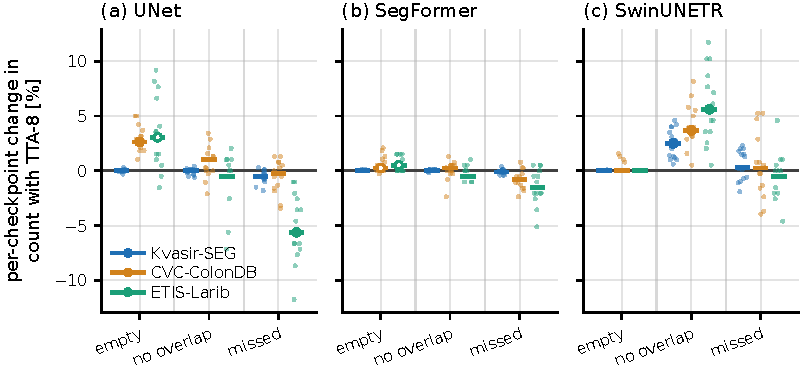
\includegraphics[width=\linewidth]{figures/fig_ckpt.pdf}}
\end{figure}

\emph{Per checkpoint.} With the checkpoint as the unit (Fig.~\ref{fig:ckpt}), 5 of the 27 cells survive Holm correction at $p<0.01$. Three are SwinUNETR's: images with no overlap rose in all 15 checkpoints on all three collections (medians $+25$, $+14$ and $+11$, Holm $p=0.002$ each) while its missed images moved in no direction on any of them (unadjusted $p=0.30$, $1.0$ and $0.39$), so within each collection, on the same predictions, one criterion says significantly harmed and the other says nothing. The other two are UNet's, and they point opposite ways in different collections: more images left empty on CVC-ColonDB in all 15 checkpoints (median $+10$ of 380) and fewer missed at IoU 0.10 on ETIS-Larib in all 15 (median $-11$ of 196). On ETIS-Larib alone UNet shows both directions at once, though only the fall survives correction, with empty predictions up in 13 of 15 checkpoints (median $+6$, $p=0.007$). SegFormer's empty predictions rose too, on CVC-ColonDB and ETIS-Larib (12 of 15 and 9 of 15, median $+1$ each, $p=0.003$ and $0.004$), short of Holm but invisible to the majority vote, which moves SegFormer by at most three images under any count, so the vote understates this model rather than inflating it. The counts below are the image-level view.

\emph{Empty predictions.} For UNet, TTA emptied predictions. On CVC-ColonDB and ETIS-Larib, the images that most UNet checkpoints left empty rose from 55 to 68 of 380 (unadjusted $p=0.002$, block bootstrap of the change $[7, 20]$) and from 5 to 18 of 196 ($p<0.001$, $[4, 23]$) with TTA-8 (Appendix~\ref{app:figs}, Fig.~\ref{fig:misses}). The counts vary widely between checkpoints (on ETIS-Larib the median left 12 images empty without TTA and 15 with it, ranges 1 to 29 and 5 to 42), so the majority vote is a summary and not the behaviour of one model. The 14 newly empty ETIS-Larib images fall into 9 runs of consecutive image numbers against 13 expected at random, so those images are probably not independent and this $p$-value is optimistic.

\emph{No overlap.} Most newly empty images already had no overlap with the polyp: of the 15 and 14 newly emptied, 12 and 11 already had none without TTA, and UNet's no-overlap counts stayed at 70 and 33, the rest being real losses of single images (Appendix~\ref{app:qualitative}). For SwinUNETR, which never predicted an empty mask on a polyp-free frame, they rose with TTA-8 from 18 to 43 of 1000 on Kvasir-SEG, from 73 to 99 on CVC-ColonDB and from 50 to 71 on ETIS-Larib ($p<0.001$ each; block bootstraps $[15, 36]$, $[16, 37]$ and $[12, 32]$), while its Dice rose by 0.006 to 0.009.

\begin{figure}[!t]
\floatconts
  {fig:sweep}
  {\caption{How the verdict on TTA depends on the bar. For each collection, the change in missed images with TTA-8 (as a percentage of the collection) against the IoU an image must reach to count as localised; 0 is the any-overlap criterion. Above the line TTA looks harmful, below it helpful. Filled markers: exact McNemar $p<0.01$, unadjusted (not Holm survivors, unlike Fig.~\ref{fig:ckpt}). Shaded band: between the last bar at which any rise is significant and the first at which none is. Counts for five of these nine thresholds are in Table~\ref{tab:criteria}.}}%
  {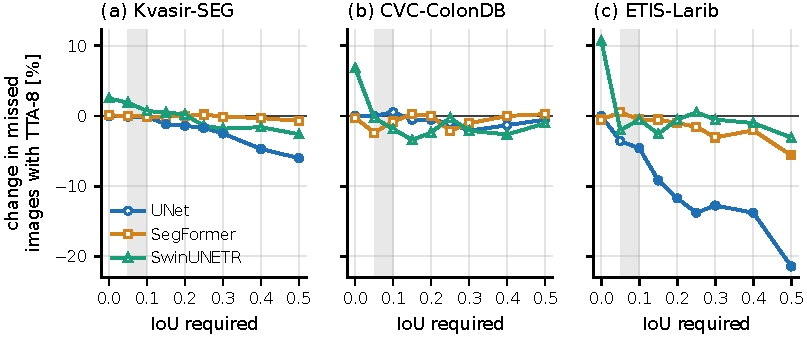
\includegraphics[width=\linewidth]{figures/fig_sweep.pdf}}
\end{figure}

\emph{Missed images.} With an IoU of at least 0.10 required, the SwinUNETR effect disappeared: missed images went from 216 to 223, 189 to 182 and 145 to 144 (the only rise at $p=0.37$; block bootstraps $[-6, 20]$, $[-21, 7]$ and $[-7, 4]$). That model had failed externally (Dice 0.14 to 0.40), and what it lost with TTA was mostly overlap that did not reach this IoU. UNet missed fewer images on ETIS-Larib with TTA-8, 46 against 55 (none newly missed, 9 recovered, $p=0.004$, $[-18, -2]$), and about as many on CVC-ColonDB (76 against 74; $[-2, 6]$) and Kvasir-SEG (26 against 27; $[-6, 3]$). SegFormer changed by at most three images under any of the three counts. The sweep says where in the grid the verdict turns (Fig.~\ref{fig:sweep}): requiring any overlap, three counts rise significantly, all SwinUNETR's; at IoU 0.05 one still does, SwinUNETR on Kvasir-SEG, a single unadjusted test on the broken model in the one collection we could not block, which we record and do not build on; from 0.10 upward none does, in any of the 63 comparisons at the seven thresholds from 0.10 to 0.50, the smallest $p$ on any rise being 0.37. We chose 0.10 after seeing the first two counts, so we cannot call it the right bar, only the lowest in our grid at which no rise survives anywhere. Above it the direction is stable and favours TTA, with UNet's falls on ETIS-Larib growing to 85 against 58 at 0.25 and 131 against 89 at 0.50 (Appendix~\ref{app:criteria}).

These are non-rejections, not demonstrations of safety: the widest interval admits about 20 more missed images per 1000, we set no non-inferiority margin, and the study was not powered to exclude a small rise. We hold the fall to the same bar we set for rises: it counts as a result because the direction repeats, at every threshold from 0.10 to 0.50 and in all 15 checkpoints, but it does not repeat across datasets, so it is a result about UNet on ETIS-Larib and not about TTA. These counts are also images and not polyps. On ETIS-Larib the 9 images UNet no longer missed fall into 7 runs of consecutive image numbers and the 14 newly empty images into 9 runs, so each stands on single-digit numbers of polyp episodes within a set holding 44 polyps, and the releases carry no polyp identities to resolve it further.

Gains by lesion size ran the other way from the losses, being smallest for UNet on the largest-polyp tertile of all three sets and negative for SwinUNETR on two of them, while the emptied predictions were not confined to the smallest polyps (Appendix~\ref{app:size}).




\subsection{Recovery rules and the operating point}
\label{sec:res-rules}
% Source: detection_rules/internal_misses.csv, external/*/misses_vs_tta8.csv,
% brats/misses.csv, brats/false_positive.csv (McNemar vs TTA-8), internal_paired.csv,
% external/*/paired.csv, brats/paired.csv; false_alarm/tables/false_alarm_all.csv.
Both rules filled most of the empty predictions and cost no mean Dice (Table~\ref{tab:rules}, Appendix~\ref{app:rules}). With either, most UNet checkpoints left 13 images empty on CVC-ColonDB and none on ETIS-Larib, against 55 and 5 without TTA and 68 and 18 with TTA-8, and missed images on CVC-ColonDB fell from 76 with TTA-8 to 52 and 65 ($p<0.001$ each). They change no non-empty mask, yet NSD fell by 0.002 to 0.008 and HD95 rose by 1.1 to 6.8\,px (Holm $p<0.01$), the survivorship effect of Section~\ref{sec:res-external} running in reverse.

The price is false alarms. The models, trained only on frames containing a polyp, fired on most polyp-free frames from another centre (Appendix~\ref{app:sanity}). On the 1009 normal cecum frames the share with a predicted polyp was 70.8\% for UNet and 96.4\% for SegFormer, which TTA-8 lowered to 56.5\% and 89.9\%; SwinUNETR marked a polyp on all 1009 frames with and without TTA, and TTA-8 only shrank the mask. This matches the downward shift of foreground probability that emptied predictions under shift: UNet's mean maximum probability on these frames fell from 0.74 to 0.59. These models never saw a frame without a polyp, so the mechanism acts on networks calibrated only on positives, and we cannot say the direction would transfer to a model trained with negative frames, which is what a deployed detector is. The rules push the rate back up, for UNet to 94.5\% and 89.5\%, and every count is monotone in $t$. The middle setting is the informative one: at $t=0.30$ the rule removed the whole empty-prediction rise, leaving 5 images empty on ETIS-Larib against 5 without TTA and 45 on CVC-ColonDB against 55, and still missed fewer images than the baseline on both sets (44 against 55 and 71 against 74), at 78.5\% false alarms against 70.8\%. That is far too high to deploy, but it is the one setting in our grid that pays for the empty predictions without giving back the gain in localisation. TTA and the rules therefore move UNet along a trade-off between empty predictions and false alarms (Fig.~\ref{fig:operating}), which for SegFormer appears only at the checkpoint level. Both rules fire on 90\% or more of normal frames, which leaves them a probe into the shape of that trade-off and not a deployable setting.

% Source: results/paper_checks/single_view_rule.csv, strict_overlap.csv, strict_overlap_transitions.csv, operating_curve.csv
% (scripts/paper_checks/single_view_rule.py; configs/cvc_clinicdb/unet_resnet50_baserules.yaml).
The lower threshold alone did not give this recovery. Applied to the single view, the rule with $t=0.20$ left no image empty on either set, but missed images barely moved, 73 and 55 against 74 and 55 without it, while firing on 96.4\% of polyp-free frames: on a single view the rule fills empty masks mostly off the polyp. The same rule on TTA-8 missed 65 and 41 at 89.5\% false alarms. After the rule a prediction is empty exactly when its maximum probability is below $t$, so each arm traces a detection curve through $t=0.5$, 0.4, 0.3 and 0.2. The arms are matched on false-alarm rate, which allows three of those four points, because the single view at $t=0.2$ (96.4\%) exceeds anything TTA-8 reaches (89.5\%). At every matched rate the two sat within one percentage point, with the sign of the gap depending on whether image-checkpoint pairs or majorities are counted, and we did not test it (Appendix~\ref{app:criteria}). We read this as consistent with a threshold change for empty outputs rather than evidence of one. The gain in missed images is separate, because it depends on where the mask lands, which a curve of whether the model outputs anything cannot measure.


